% !TeX root = ../libro.tex
% !TeX encoding = utf8
\chapter{Figuras adicionales}\label{ap:apendice4}
\section{Mesh models visualization}
The following figures comprise a series of grids as a function of time and for several 1 $\msun$ models in which on the one hand, the evolution of surface \isotope[7]{Li} abundance relative to \isotope[1]{H} for both variable magnetic field intensities and angular velocities and on the other hand, the evolution of surface rotational velocity are shown.

\begin{figure*}
	\centering
	\begin{subfigure}[h]{0.47\textwidth}
		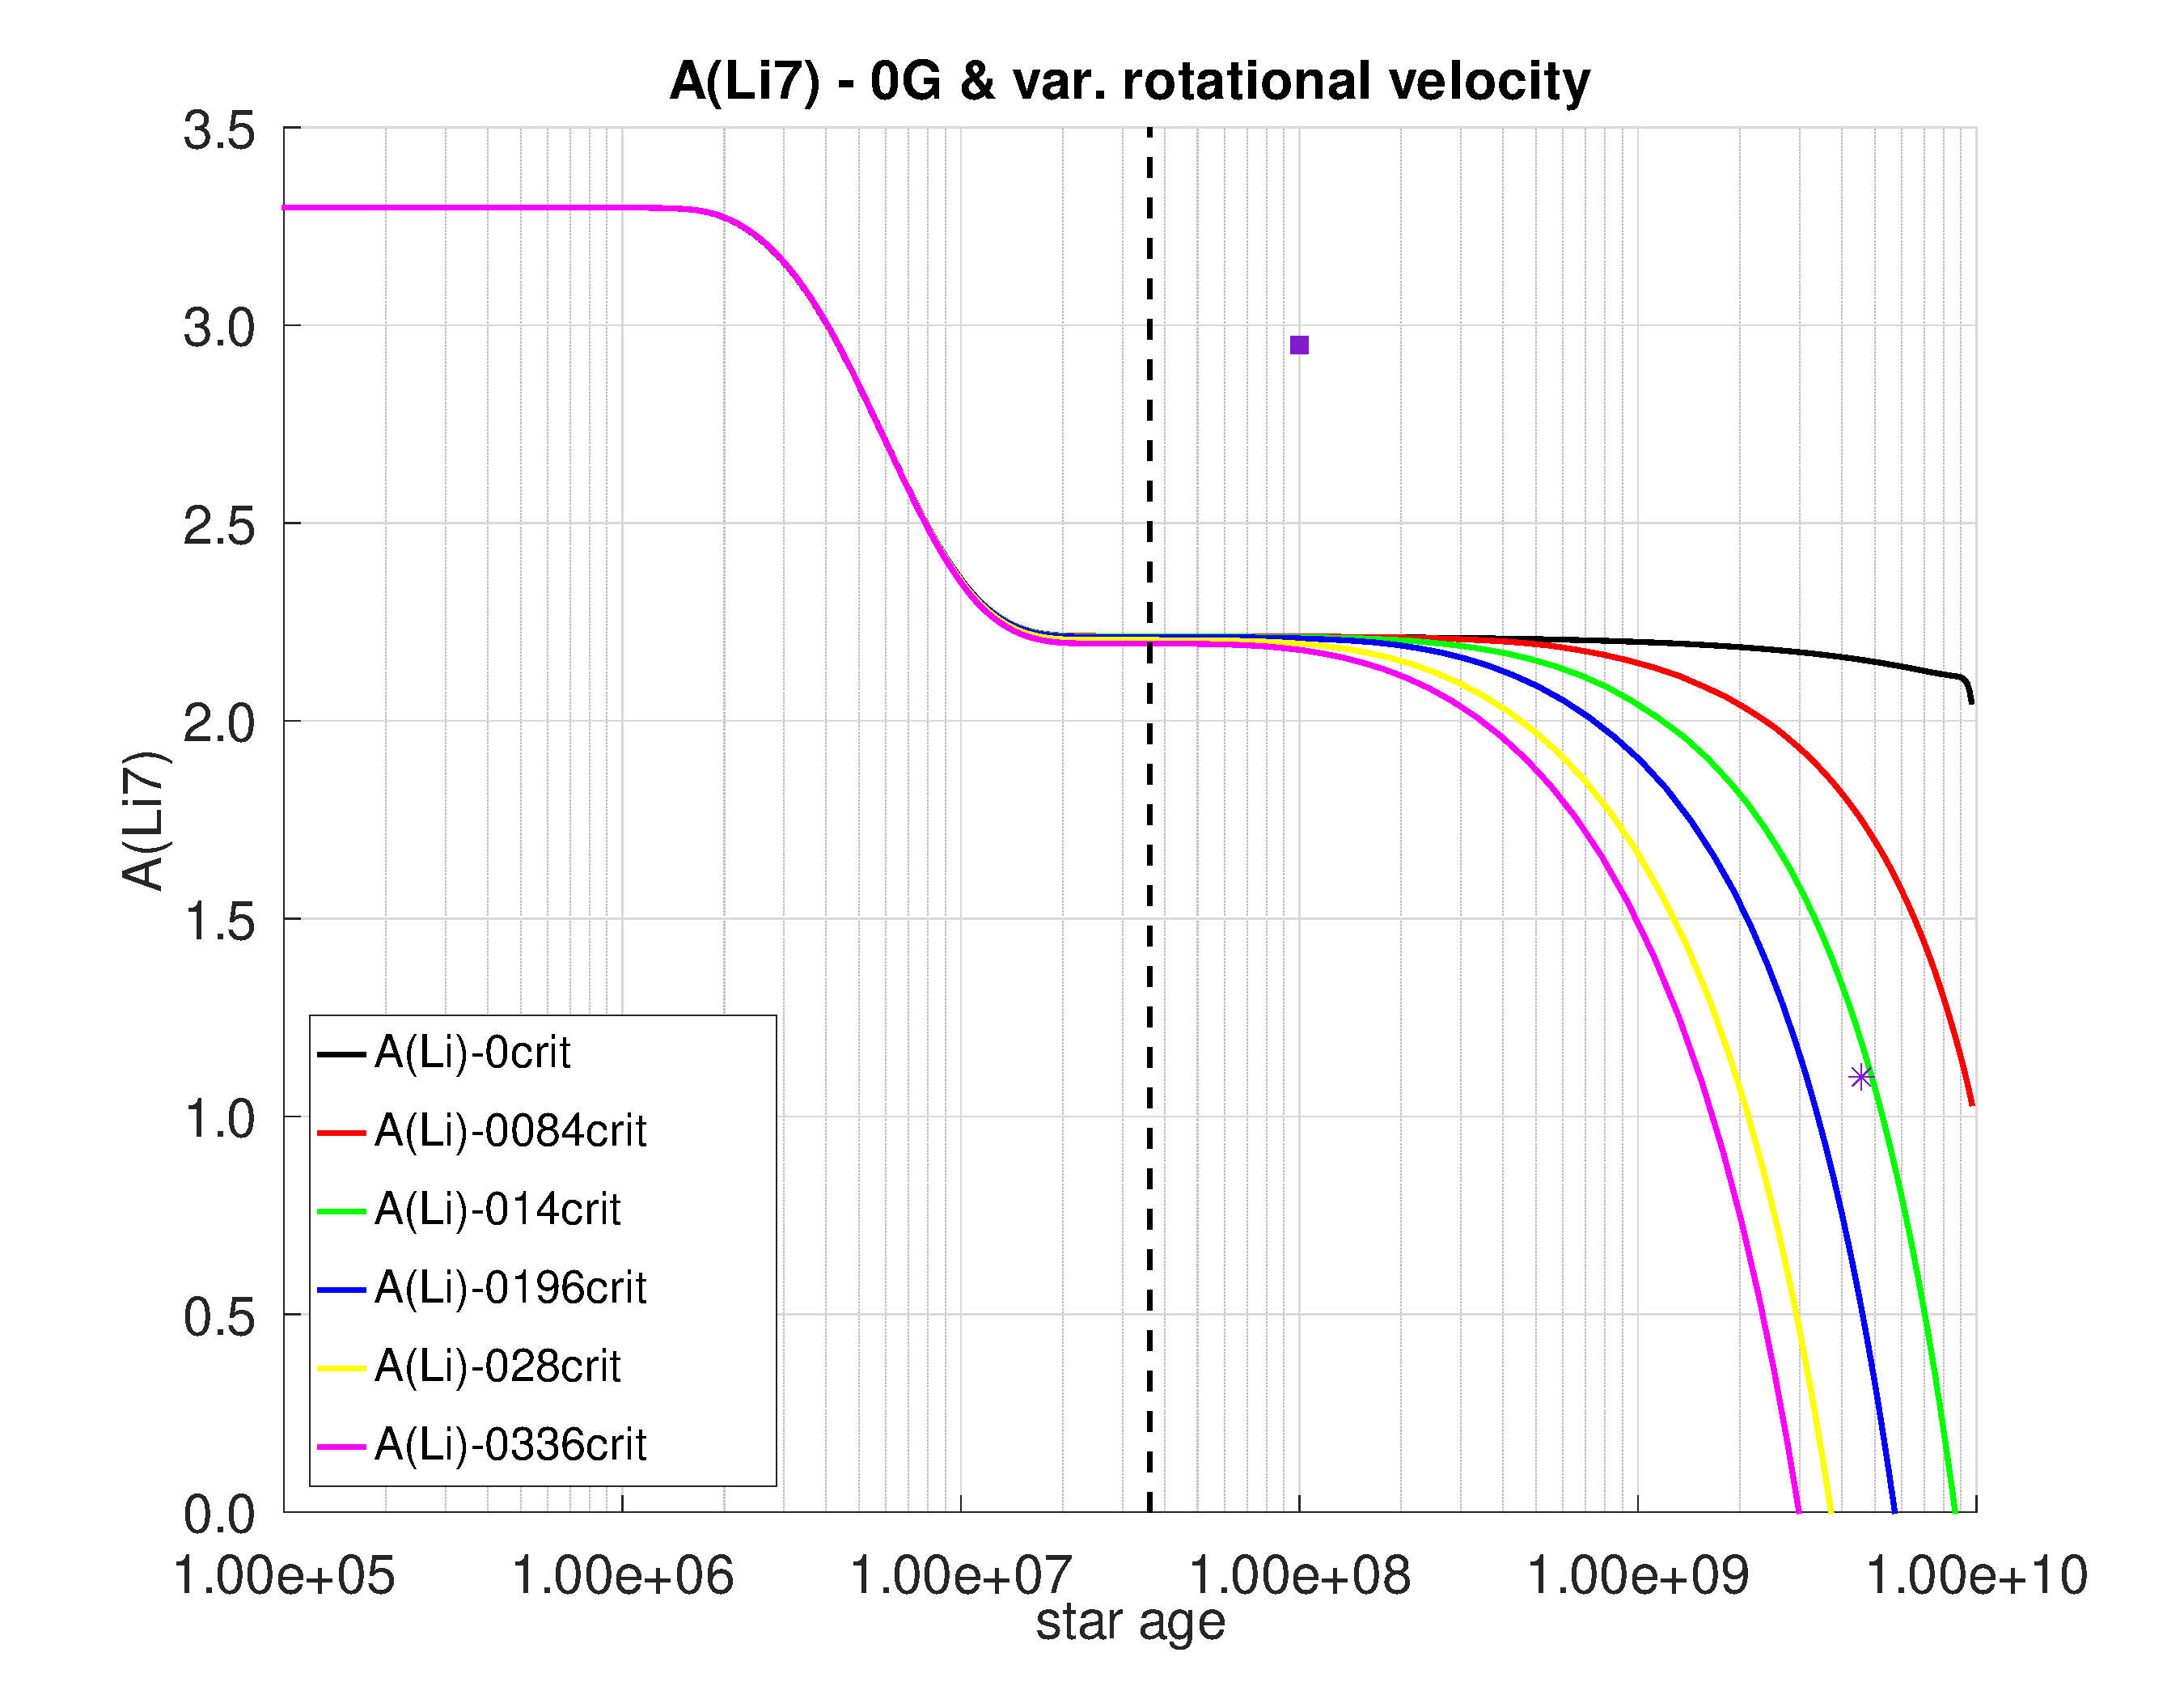
\includegraphics[trim = 25mm 10mm 15mm 10mm, clip,width=\textwidth]{img/paper1/li_var_vel_0_0g.pdf}
		\label{fig:subim1}
	\end{subfigure}
	\begin{subfigure}[h]{0.47\textwidth}
		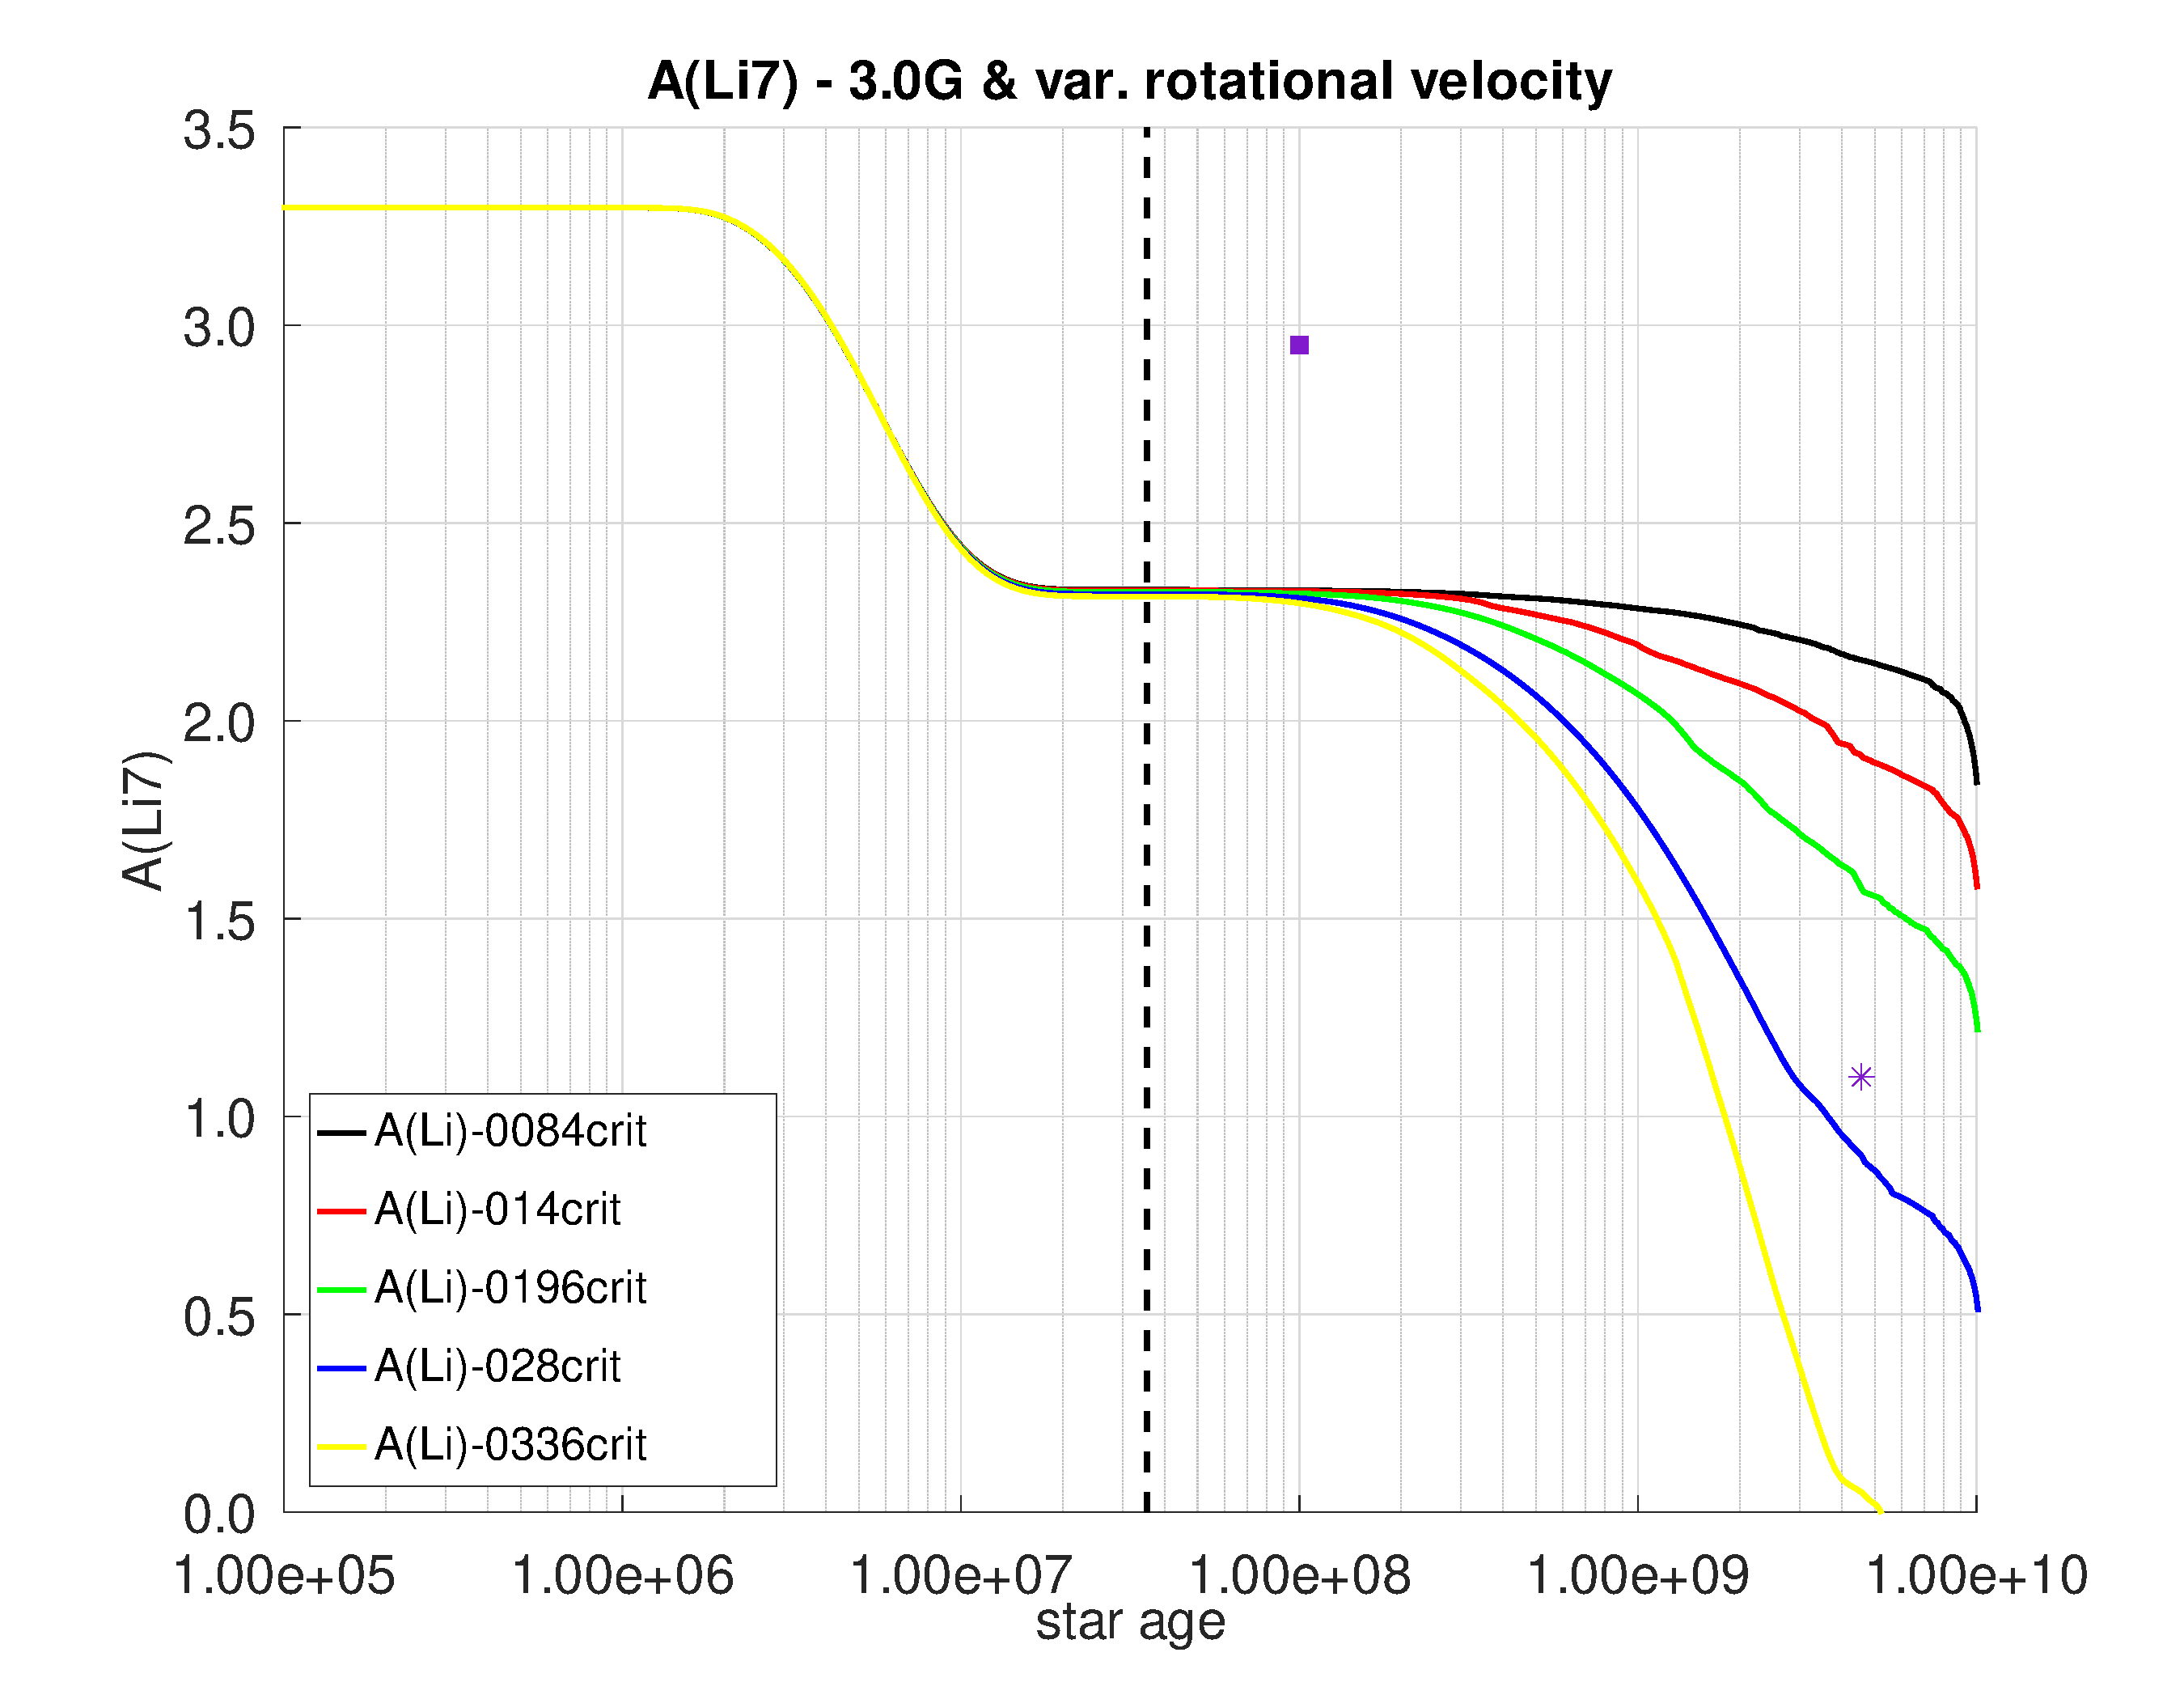
\includegraphics[trim = 25mm 10mm 15mm 10mm, clip,width=\textwidth]{img/paper1/li_var_vel_3_0g.pdf}
		\label{fig:subim2}
	\end{subfigure}
	\begin{subfigure}[h]{0.47\textwidth}
		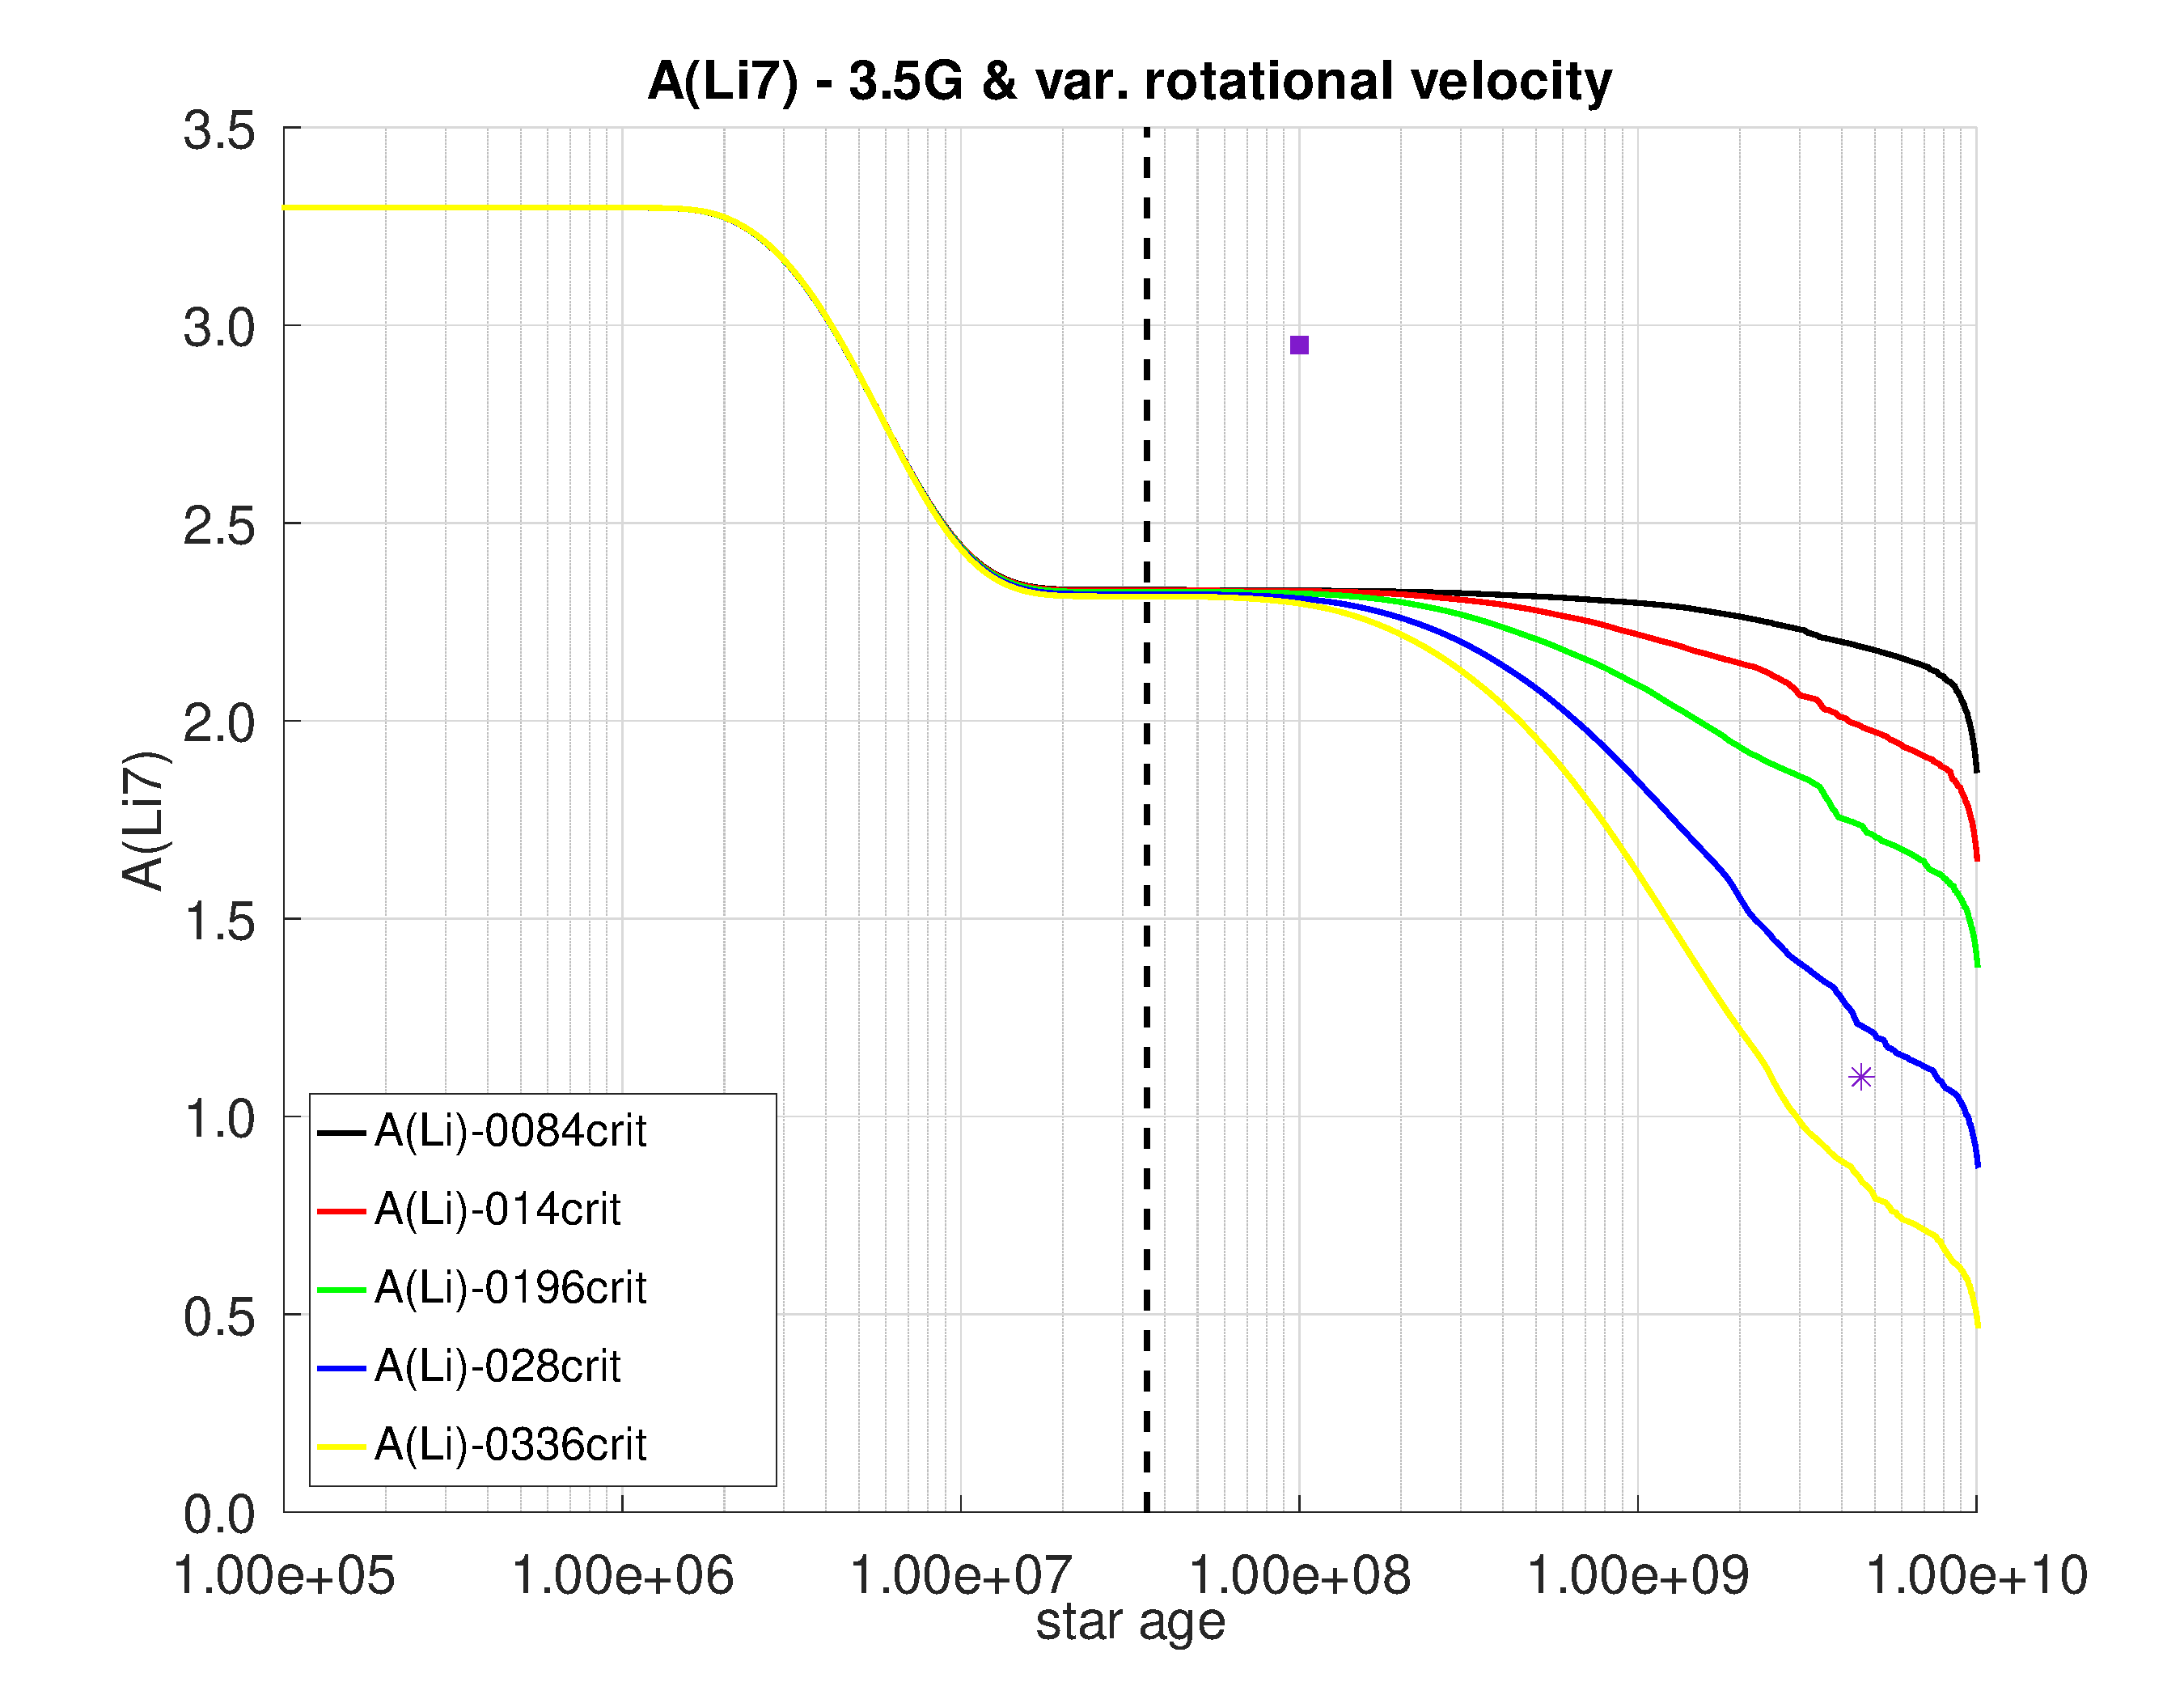
\includegraphics[trim = 25mm 10mm 15mm 10mm, clip,width=\textwidth]{img/paper1/li_var_vel_3_5g.pdf}
		\label{fig:subim3}
	\end{subfigure}
	\begin{subfigure}[h]{0.47\textwidth}
		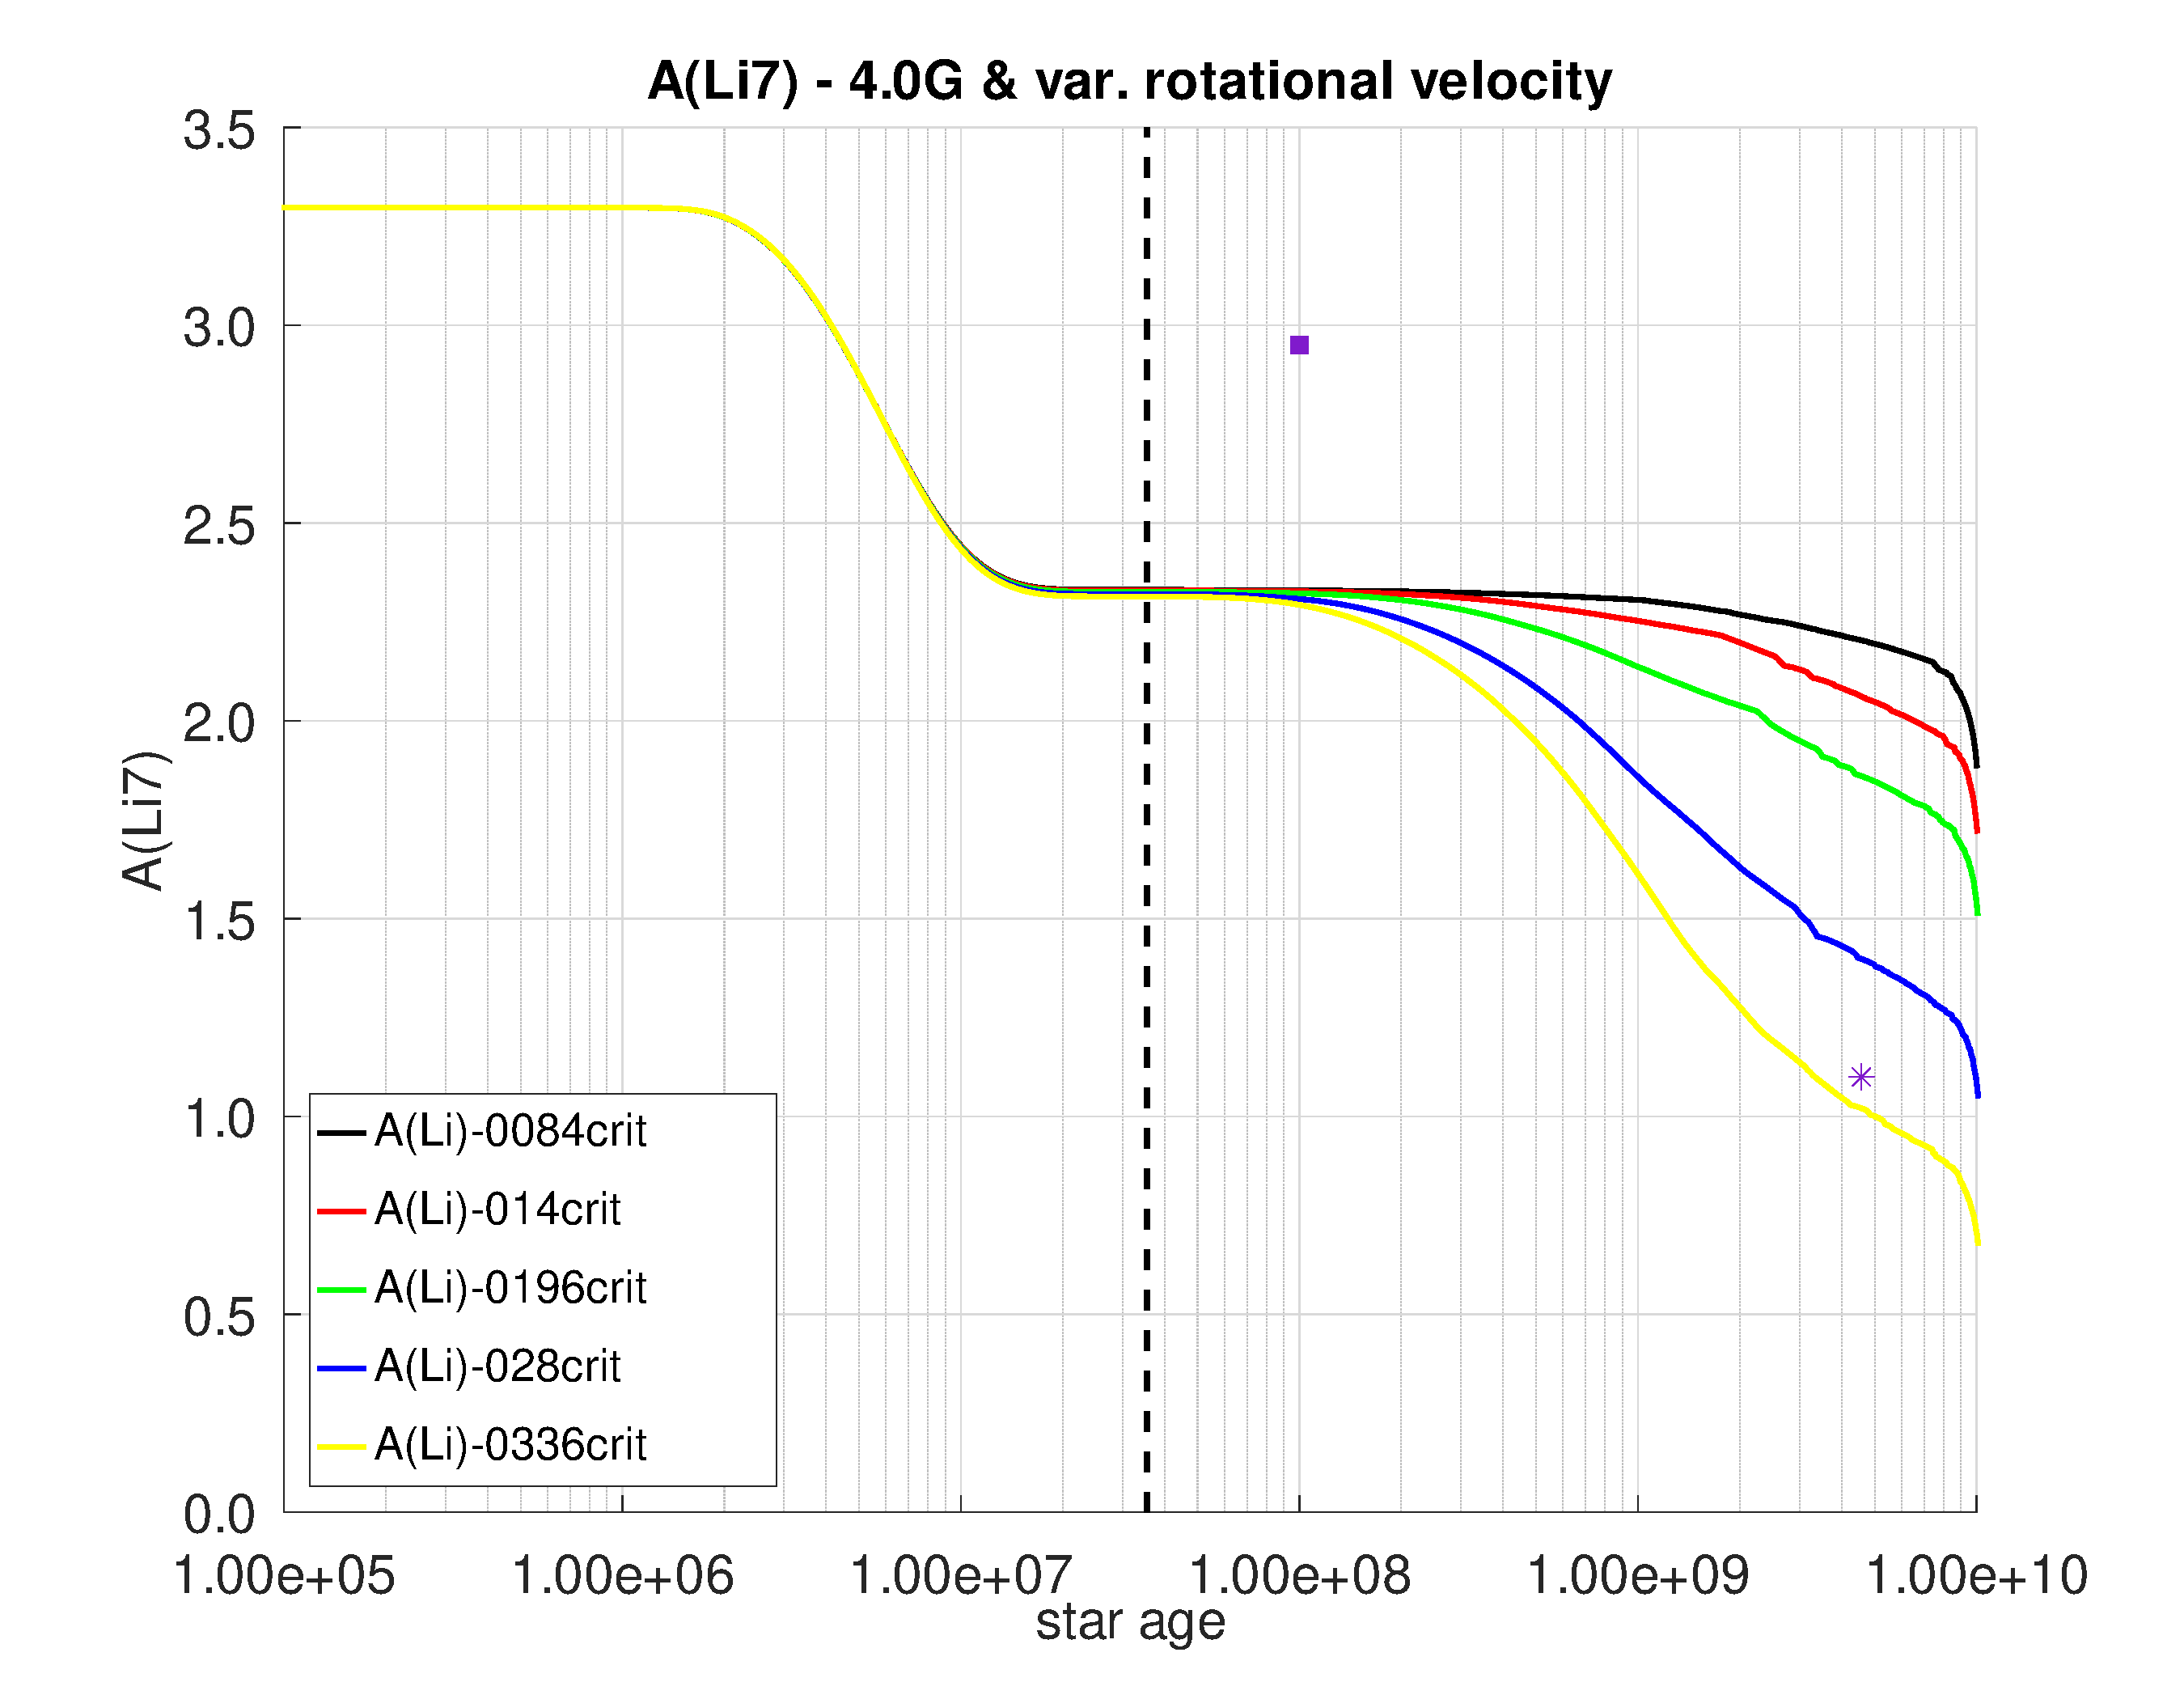
\includegraphics[trim = 25mm 10mm 15mm 10mm, clip,width=\textwidth]{img/paper1/li_var_vel_4_0g.pdf}
		\label{fig:subim4}
	\end{subfigure}
	\begin{subfigure}[h]{0.47\textwidth}
		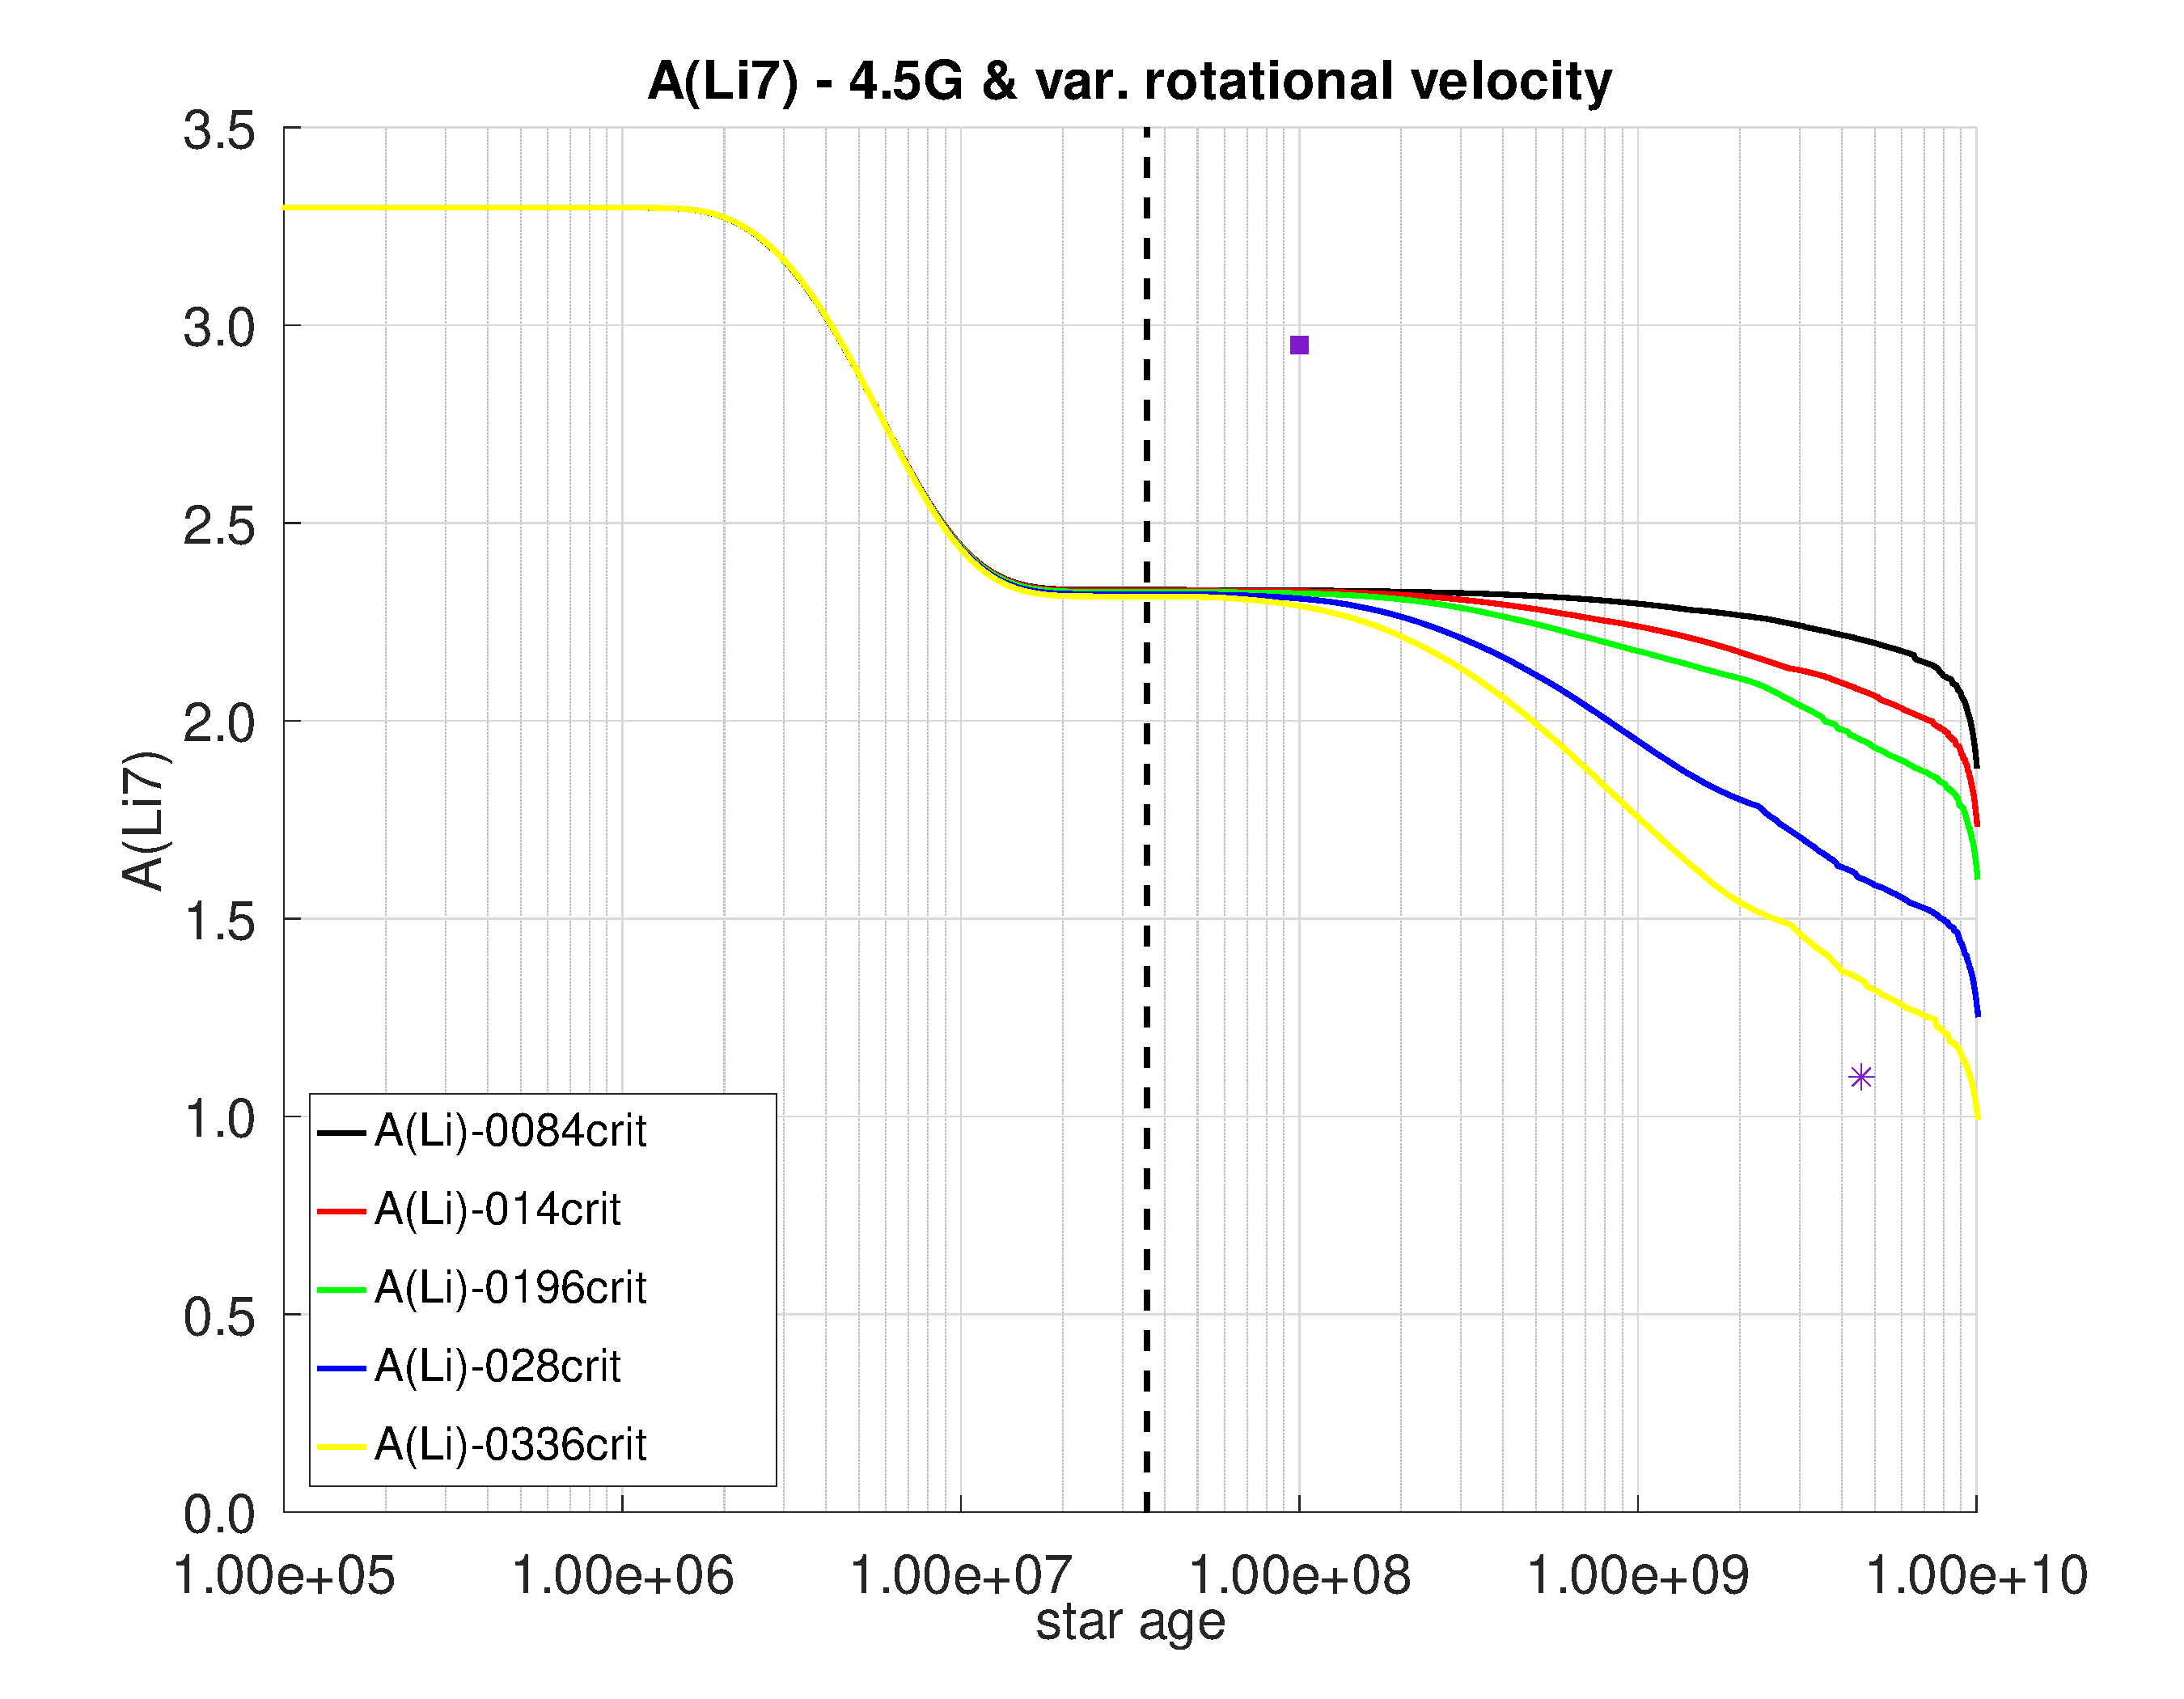
\includegraphics[trim = 25mm 10mm 15mm 10mm, clip,width=\textwidth]{img/paper1/li_var_vel_4_5g.pdf}
		\label{fig:subim5}
	\end{subfigure}
	\begin{subfigure}[h]{0.47\textwidth}
		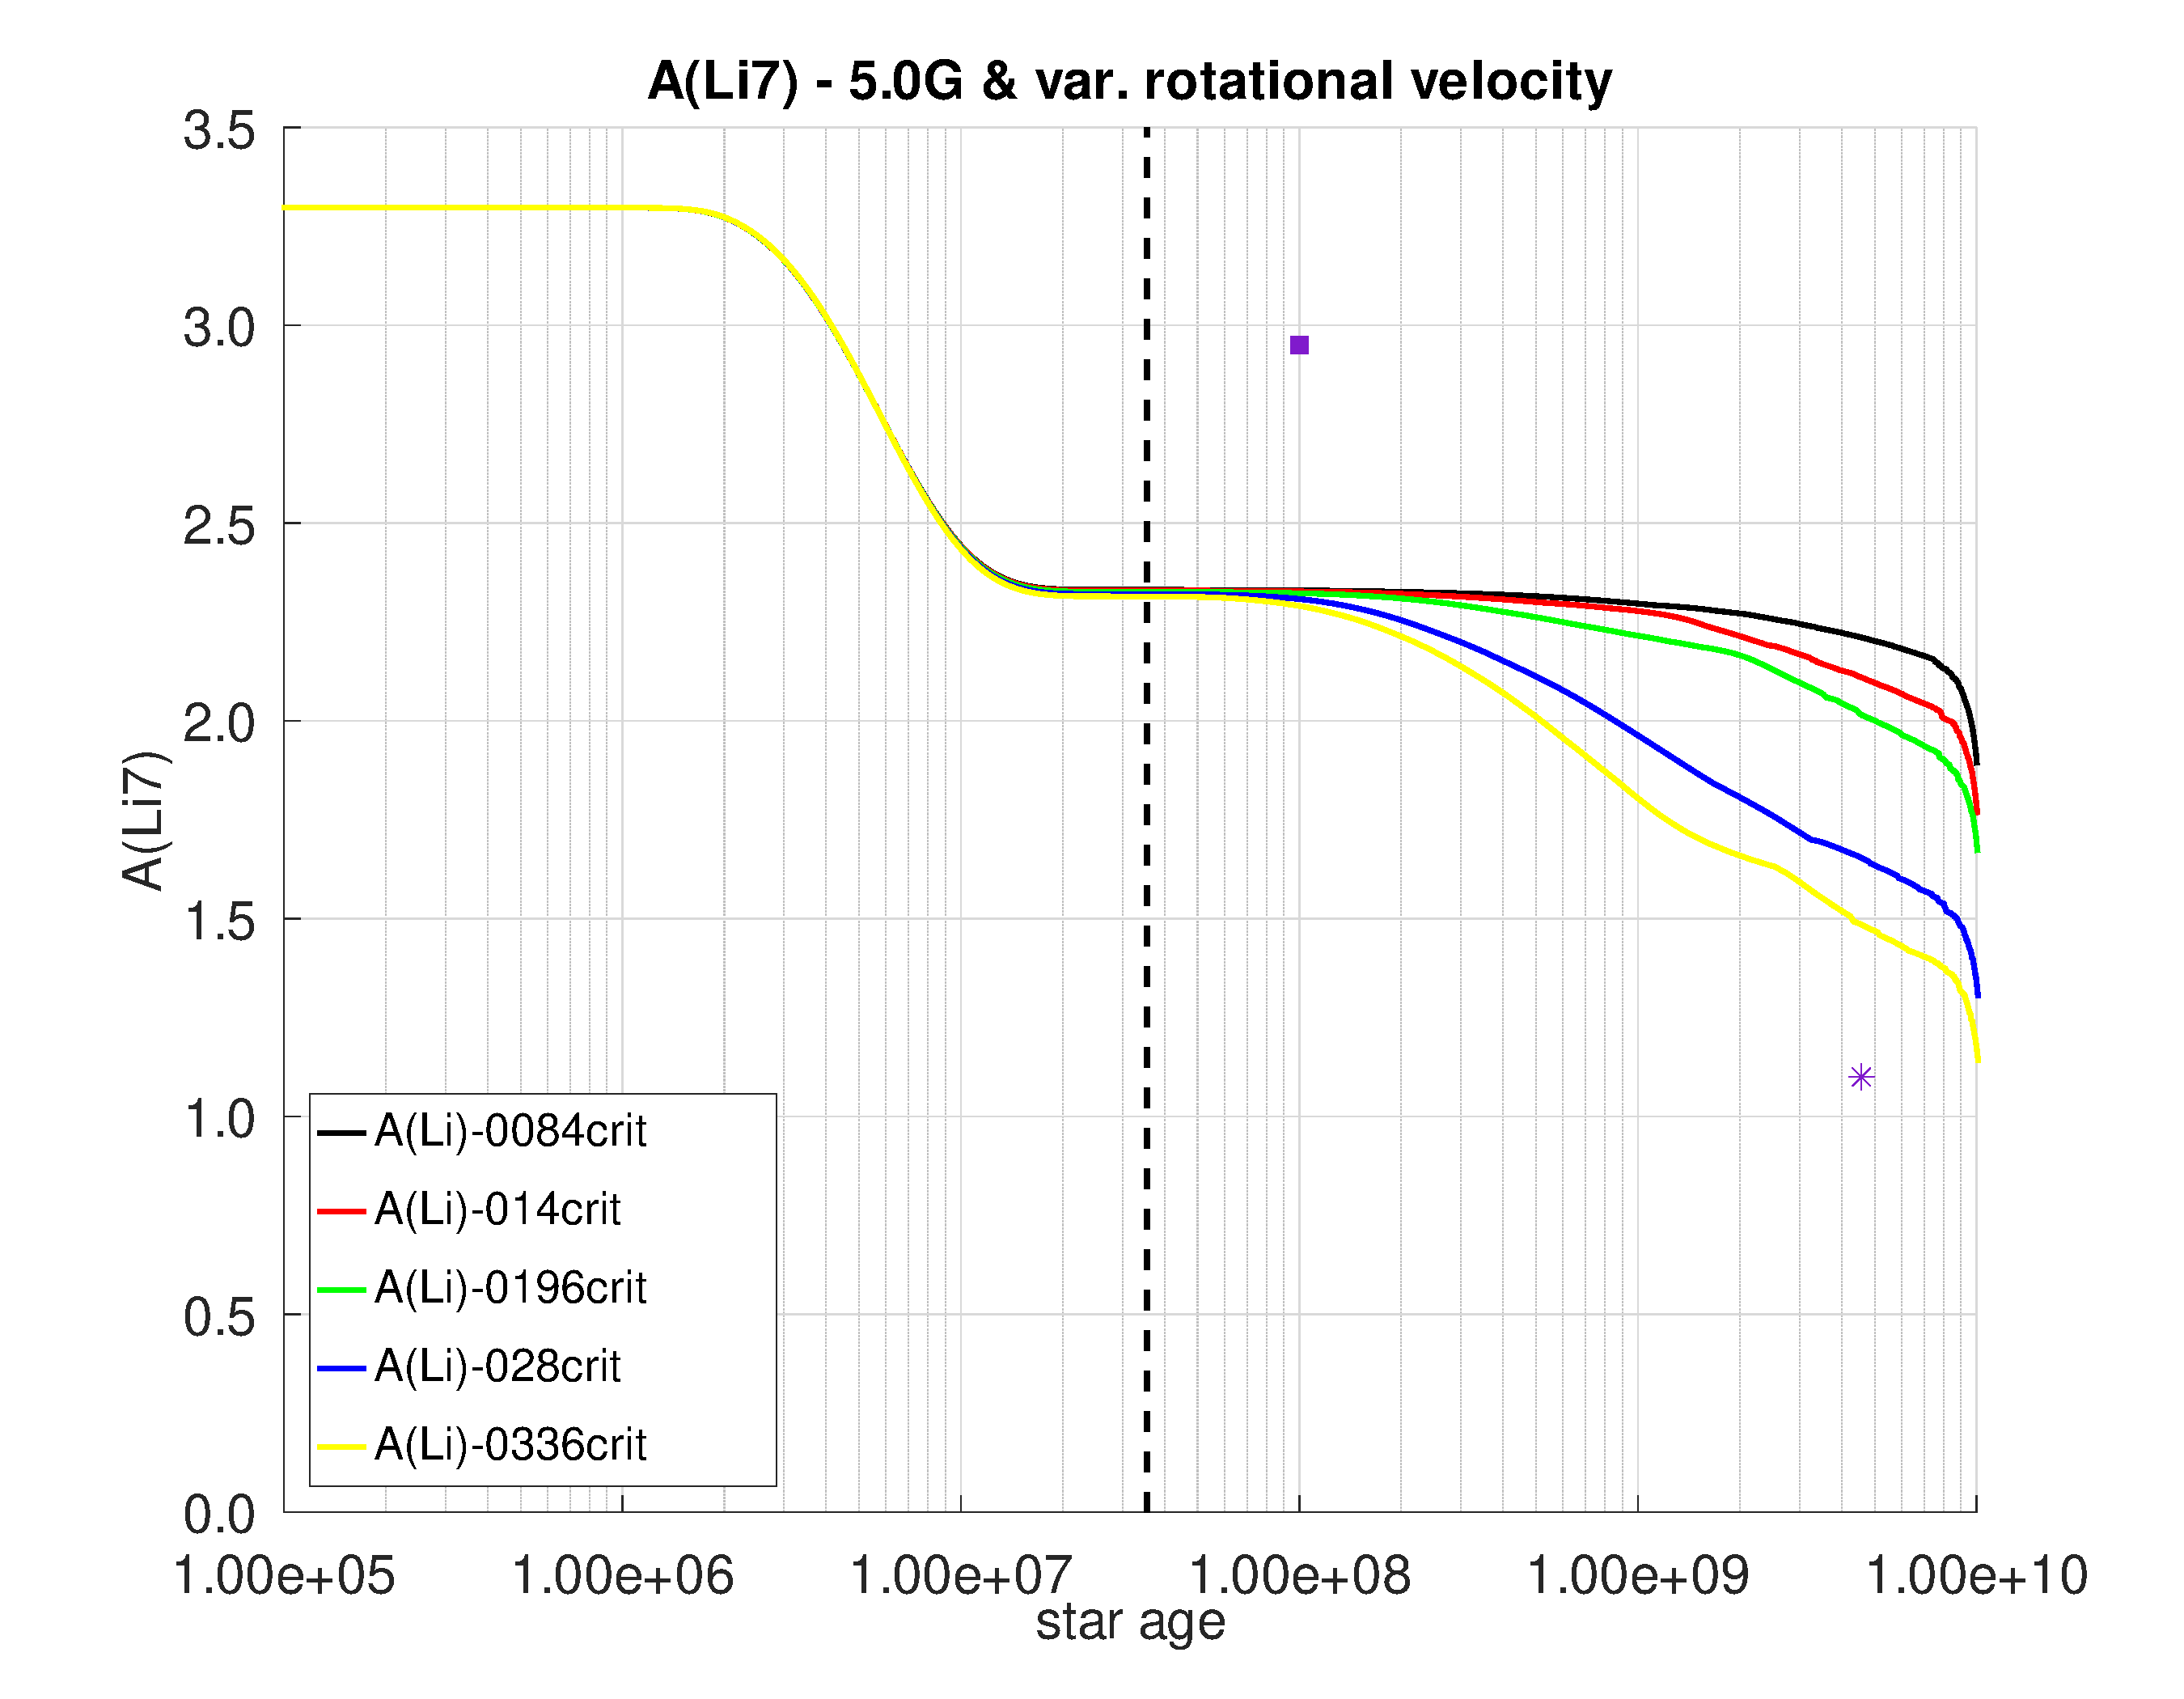
\includegraphics[trim = 25mm 10mm 15mm 10mm, clip,width=\textwidth]{img/paper1/li_var_vel_5_0g.pdf}
		\label{fig:subim6}
	\end{subfigure}
	\caption{Grid showing the evolution of surface \isotope[7]{Li} abundance relative to \isotope[1]{H}, as a function of time for several 1 $\msun$ models. Each figure shows a set of models in which the magnetic field with intensity has been fixed and $\oomegac$ varies between 0.0084 and 0.0336, respectively. The purple star and square are surface Li abundance for the present-day Sun \citep{Asplund2009} and the Pleiades cluster \citep{Sestito2005} respectively. The dashed vertical line makes reference to the ZAMS.}
	\label{fig:grid_li_var_vel}
\end{figure*}


The following figures comprise a series of grids as a function of time and for several 1 $\msun$ models in which on the one hand, the evolution of surface \isotope[7]{Li} abundance relative to \isotope[1]{H} for both variable magnetic field intensities and angular velocities and on the other hand, the evolution of surface rotational velocity are shown.

\begin{figure*}
	\centering
	\begin{subfigure}[h]{0.47\textwidth}
		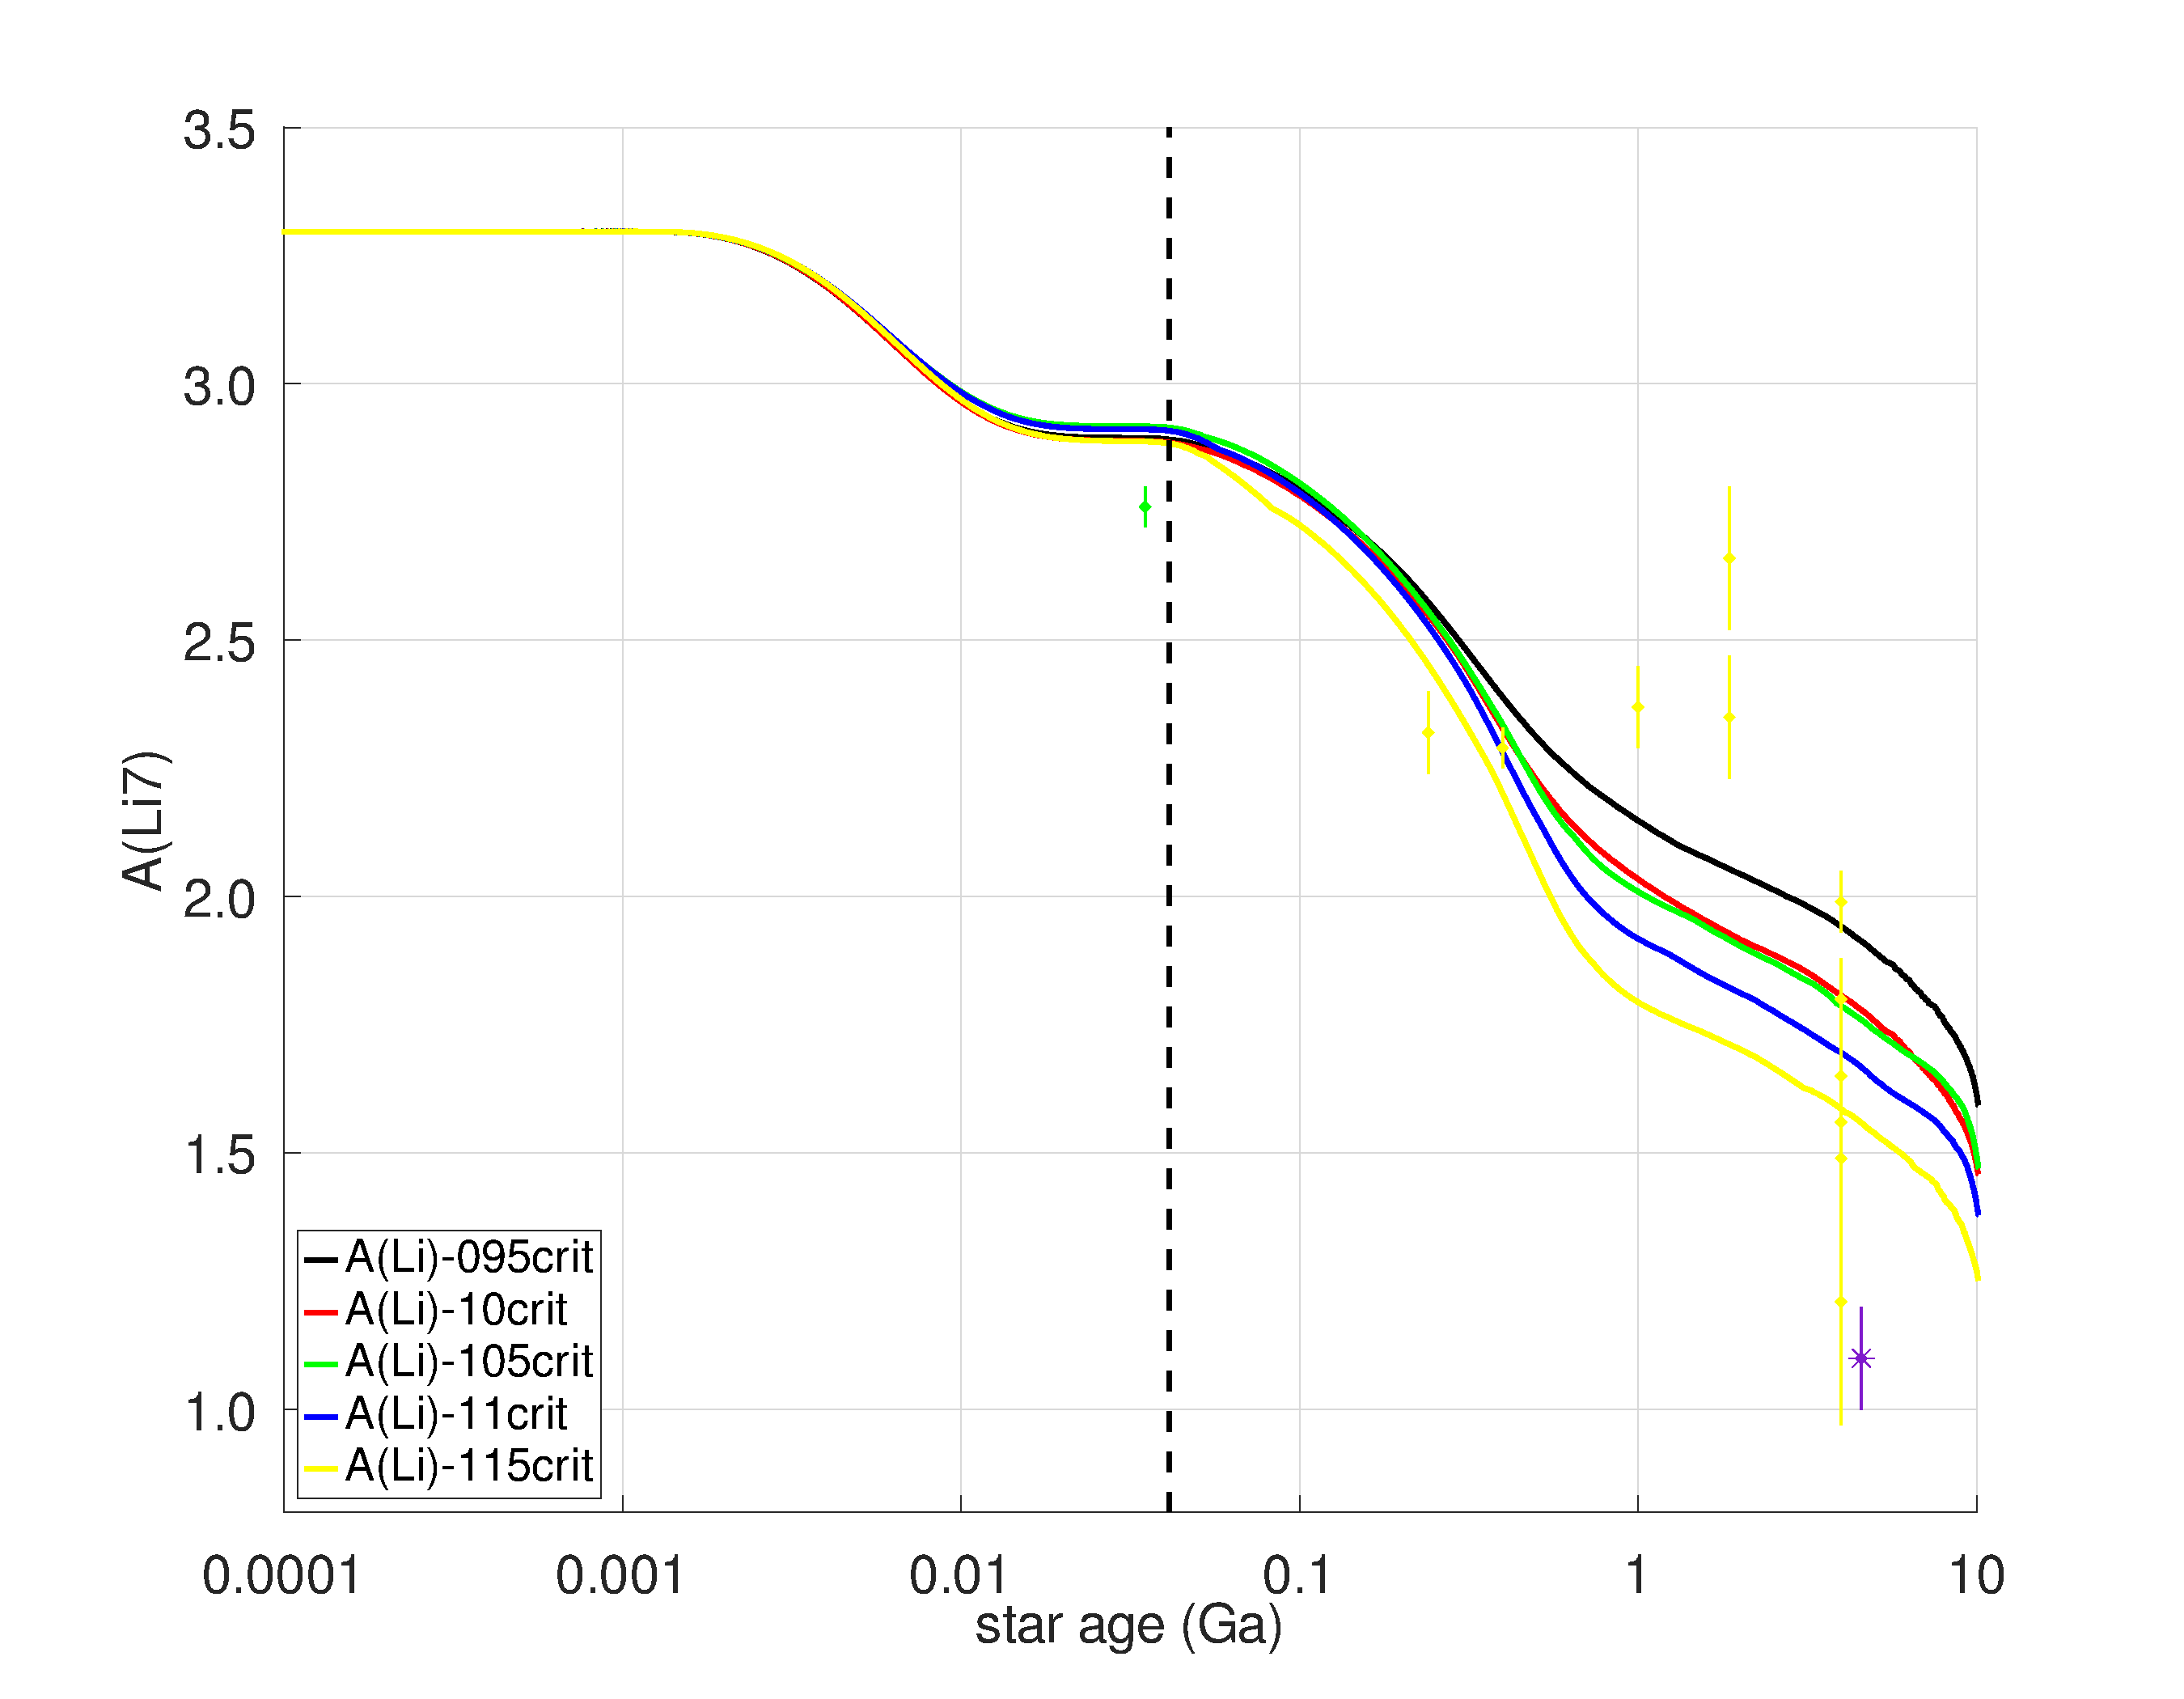
\includegraphics[clip,width=\textwidth]{img/paper2/li_var_vel_var_g_1.pdf}
		\label{fig:subim11}
	\end{subfigure}
	\begin{subfigure}[h]{0.47\textwidth}
		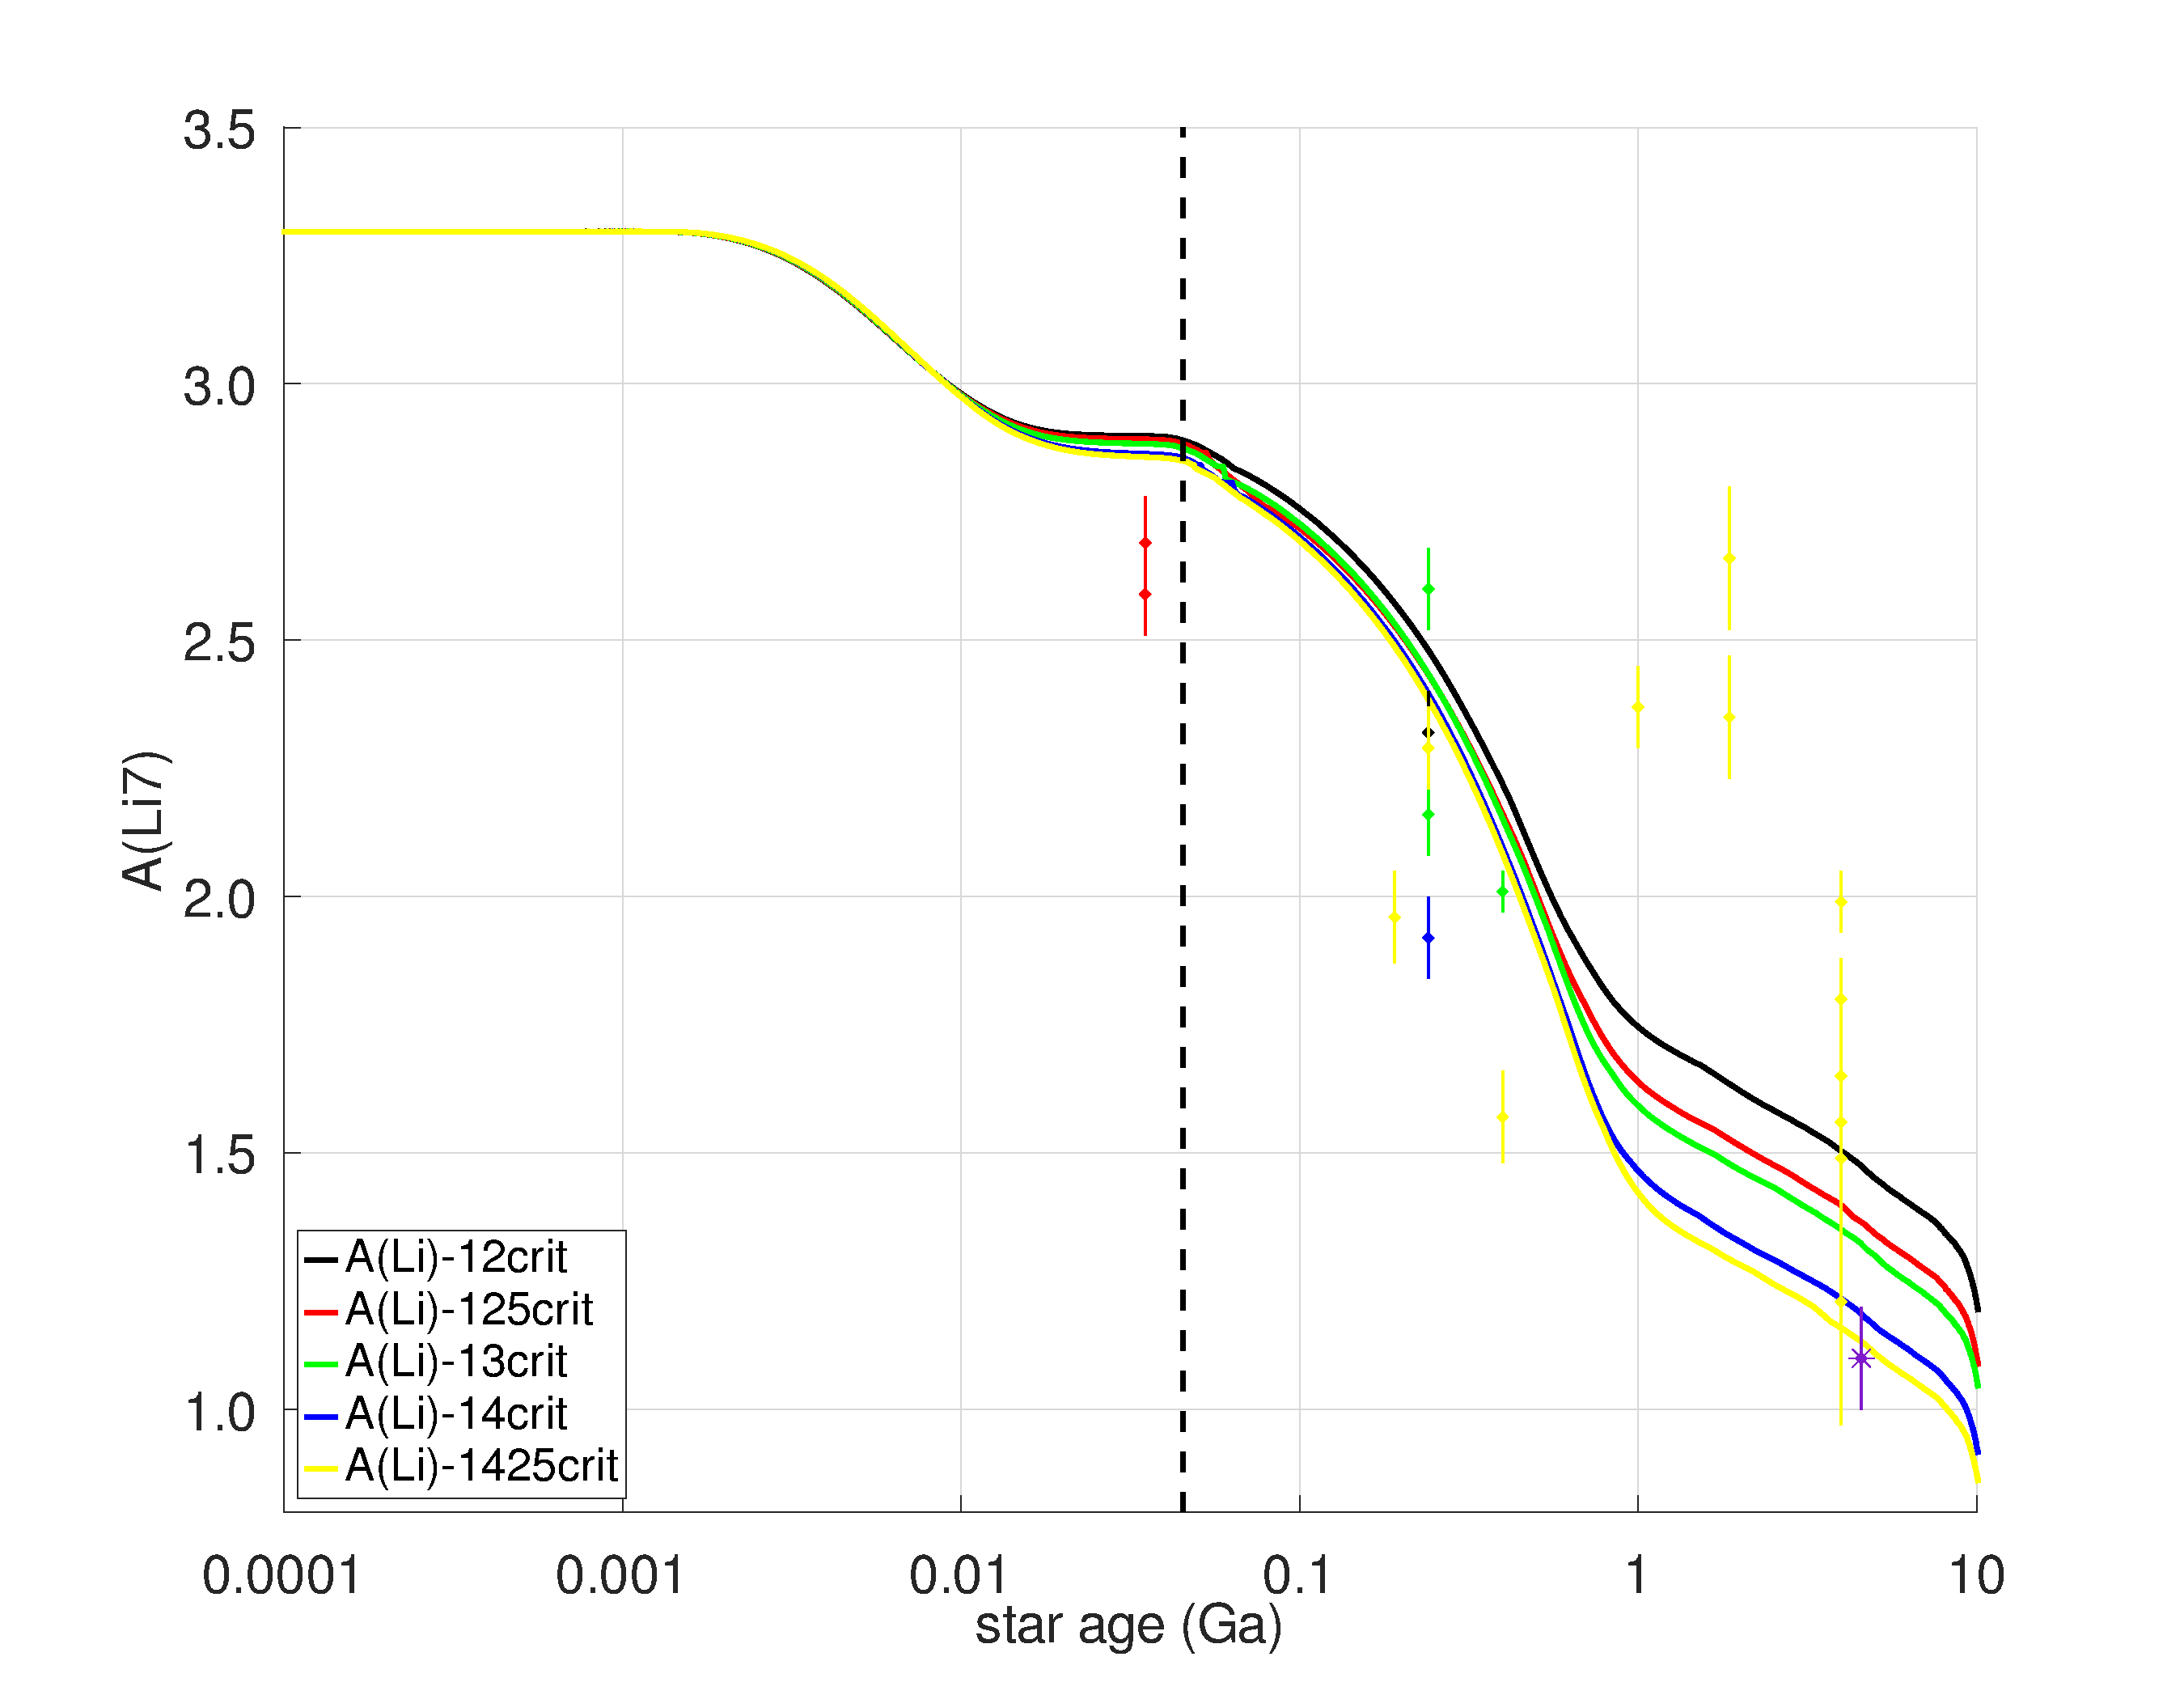
\includegraphics[clip,width=\textwidth]{img/paper2/li_var_vel_var_g_3.pdf}
		\label{fig:subim12}
	\end{subfigure}
	\begin{subfigure}[h]{0.47\textwidth}
		
\includegraphics[clip,width=\textwidth]{img/paper2/li_var_vel_0_0g_0.pdf}
		\label{fig:subim13}
	\end{subfigure}
	\begin{subfigure}[h]{0.47\textwidth}
		
\includegraphics[width=\textwidth]{img/blank.eps}
		\label{fig:subim14}
	\end{subfigure}
	
	\caption{Grid showing the evolution of surface \isotope[7]{Li} abundance relative to \isotope[1]{H}, as a function of time for several 1 $\msun$ models. Each figure shows a set of models in which the magnetic field with intensity has been fixed and $\oomegac$ varies between 0.0084 and 0.0336, respectively. The purple star and square are surface Li abundance for the present-day Sun \citep{Asplund2009} and the Pleiades cluster \citep{Sestito2005} respectively. The dashed vertical line makes reference to the ZAMS.}
	\label{fig:grid_li_var_vel}
\end{figure*}

\begin{figure*}
	\centering
	\begin{subfigure}[h]{0.47\textwidth}
		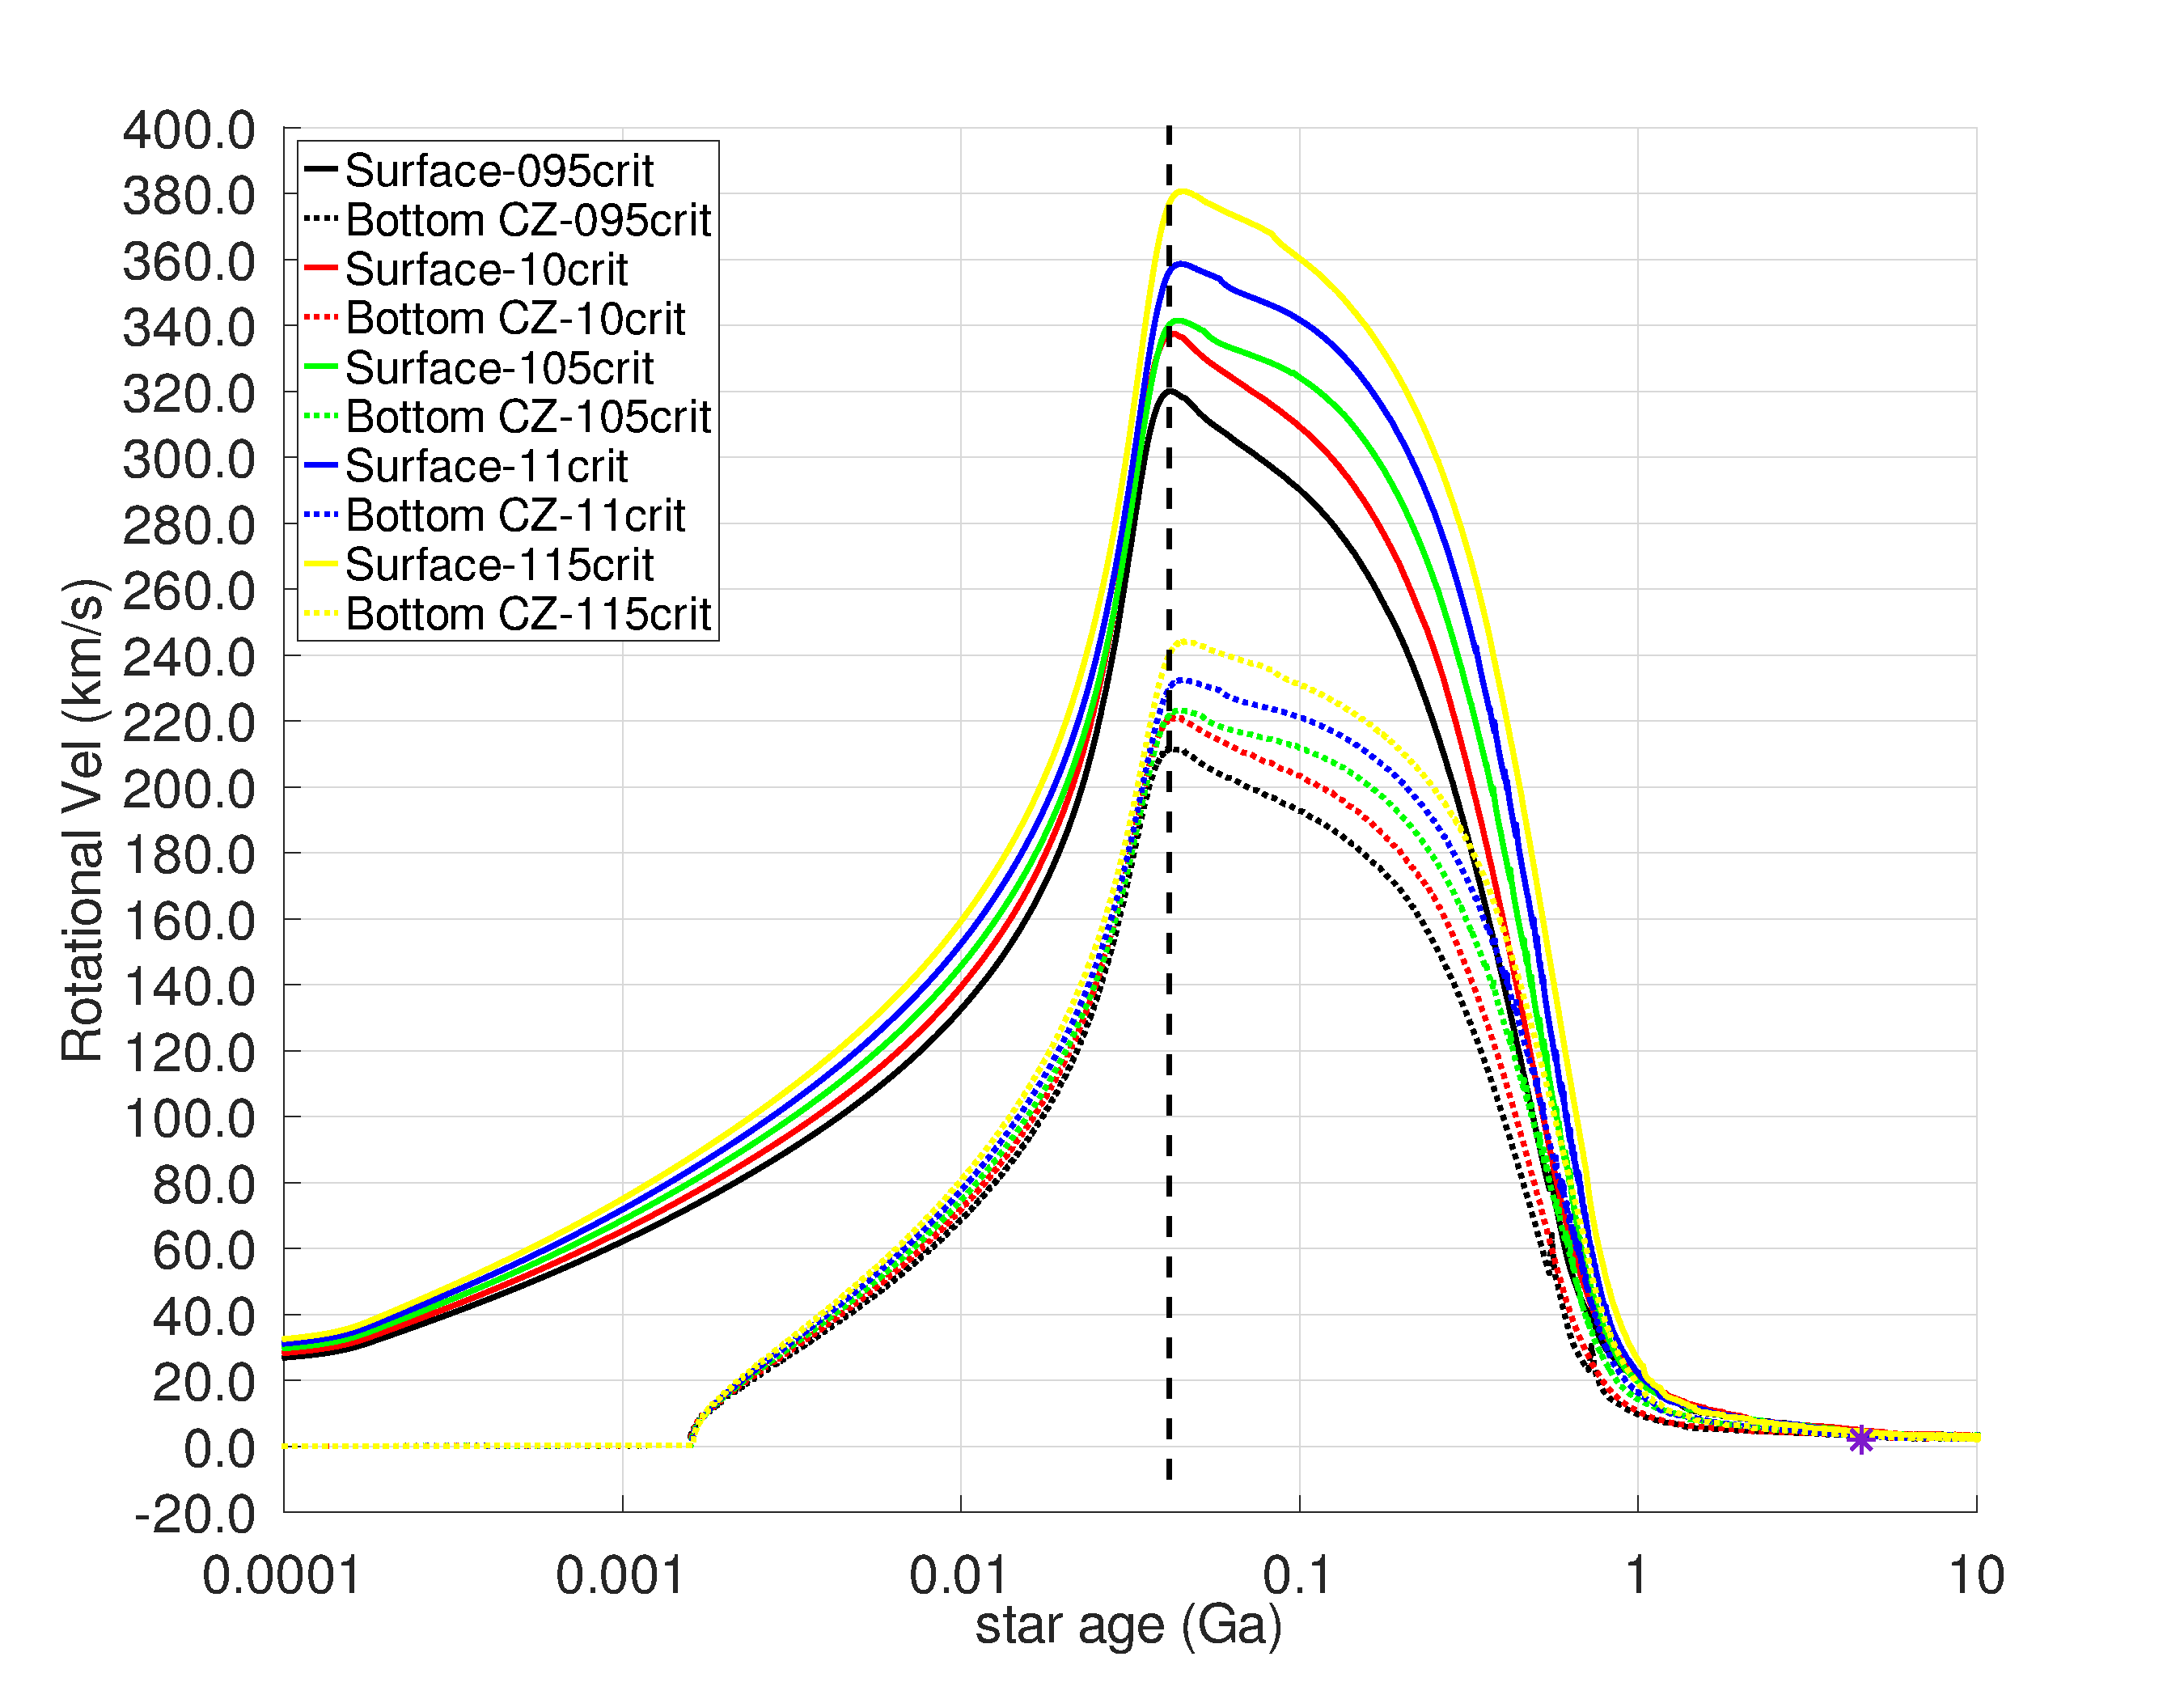
\includegraphics[clip,width=\textwidth]{img/paper2/rot_vel_var_vel_var_g1.pdf}
		\label{fig:subim21}
	\end{subfigure}
	\begin{subfigure}[h]{0.47\textwidth}
		
\includegraphics[clip,width=\textwidth]{img/paper2/rot_vel_var_vel_0_0g_0.pdf}
		\label{fig:subim22}
	\end{subfigure}    
	\caption{Grid showing of the evolution of surface rotational velocity, as a function of time for several 1 $\msun$ models. The left figure show a set of models with variable magnetic field with intensity, and $\omegaini$ varying between 0.095 and 0.115. In the right one the magnetic field intensity was set to $0.0\,\Gauss$, and $\omegaini$ varying between 0.0 and 0.0336. The purple star and square are surface Li abundance for the present-day Sun \citep{Asplund2009}. The dashed vertical line makes reference to the ZAMS.}
	\label{fig:grid_li_var_g}
\end{figure*}

\endinput
%------------------------------------------------------------------------------------
% FIN DEL APÉNDICE. 
%------------------------------------------------------------------------------------
